\section{Model Preparation}
\subsection{Data Processing}
\subsubsection{Data Filtering and Classification}
In order to better predict the momentum of the athletes, we analyzed and filtered the data.The filtered data is divided into five categories: on-court situation, special scoring ability, turnover, fitness, and serve, as shown by Figure \ref{fig:WeightP1}.
\begin{figure}[bt!]
    \centering
    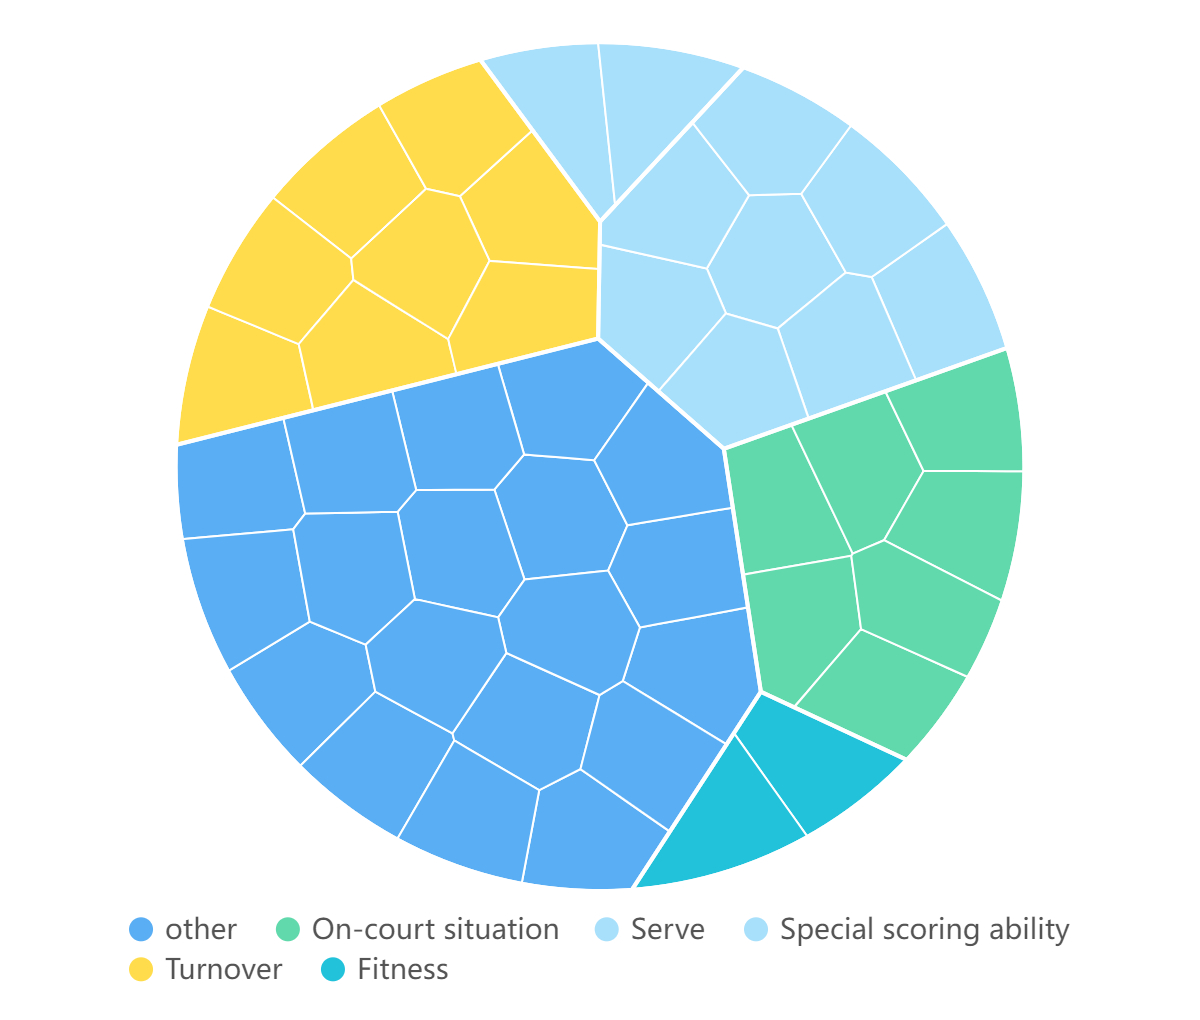
\includegraphics[width=0.5\linewidth]{figure/维诺图-副本.jpg}
    \caption{\centering Data Classification Graph}
    \label{fig:WeightP1}
\end{figure}
\subsubsection{Statistical Processing of Data}
In the raw data, there are many bool type data, which represent the events that occurred at this moment, such as aces, breaks, winners, etc., and we have statistically processed these data in order to use these data more intuitively when predicting athlete momentum. 
\begin{itemize}
    \item For special scoring ability type data, we convert a player's ace, winner score, and break score into ace rate, score winner rate, and break success rate, as shown in Figure \ref{fig:Sdeal1}.
\begin{figure}[bt!]
    \centering
    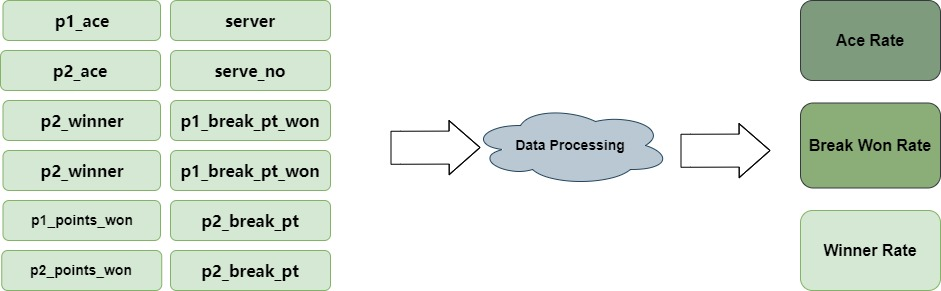
\includegraphics[width=0.75\linewidth]{figure/特殊得分数据.jpg}
    \caption{\centering Special Scoring Ability Data Transformation}
    \label{fig:Sdeal1}
\end{figure}

    \item For the error data, the number of double faults and net errors is converted into double fault service rate and net error rate through statistical methods. For the number of unforced errors, the effect on athletes' momentum was quantified by a cumulative method. Figure \ref{fig:Edeal} shows the schematic diagram of the above data conversion.
    \begin{figure}[bt!]
        \centering
        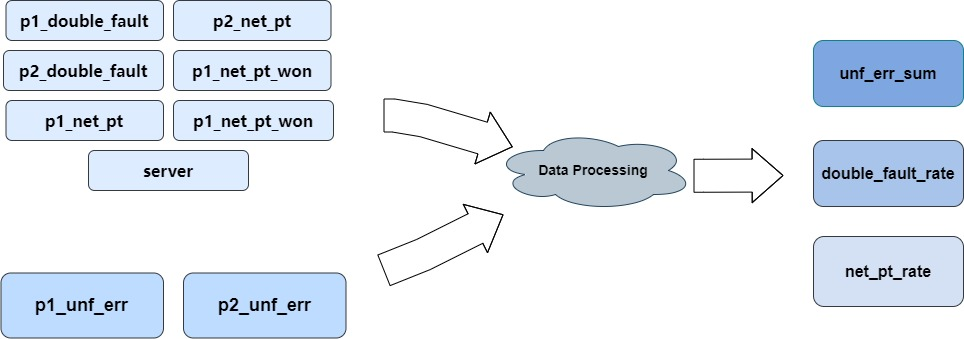
\includegraphics[width=0.75\linewidth]{figure/失误数据.jpg}
        \caption{\centering Schematic Diagram of the Error Data Conversion}
        \label{fig:Edeal}
    \end{figure}
    \item For serve data, we chose the speed of the serve, the side of the serve, and the number of serves. We mapped the serve side along with the number of serves to better quantify the impact on the player's momentum, as shown in Figure \ref{fig:Sdeal}.
    \begin{figure}[bt!]
        \centering
        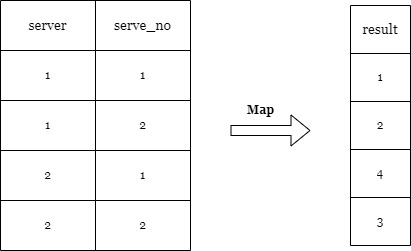
\includegraphics[width=0.5\linewidth]{figure/发球数据.jpg}
        \caption{\centering Serve Data Mapping}
        \label{fig:Sdeal}
    \end{figure}
    \item For fitness data, we add up the distance the athlete has run, and the longer the distance run, the more the athlete's momentum.
\end{itemize}
\subsubsection{Data Cleansing}
\begin{itemize}
    \item In order to make it easier to operate, the AD data in the score column is converted to 50 for subsequent operations
    \item For some missing data, such as serve speed, linear interpolation is used to supplement it.
\end{itemize}




